\documentclass[12pt]{article}

\usepackage{amsmath, color}
\usepackage{mdwmath}
\usepackage{amssymb, epsf, epsfig, textcomp}
\renewcommand{\baselinestretch}{1.3}
\usepackage{a4wide}
\newcommand{\argmin}{\mathop{\mathrm{argmin}}}
\usepackage{caption}
\usepackage{subcaption}
\usepackage{mathtools}

\usepackage{amsmath}	% Align equations: align, gather
\usepackage{amssymb}	% Math symbols: http://milde.users.sourceforge.net/LUCR/Math/mathpackages/amssymb-symbols.pdf
\newcommand\numberthis{\addtocounter{equation}{1}\tag{\theequation}}	% Number any line of an equation, can be used at end of align*

\usepackage{enumitem}	% Custom enumeration: [label=(\arabic*)], [label=(\roman*)]
\usepackage{moreenum}	% Custom enumeration: [label=(\greek*)]
\usepackage{tcolorbox}
\usepackage{listings}
\lstdefinestyle{myCustomMatlabStyle}{
	basicstyle=\ttfamily\footnotesize,
	breaklines=true,
	language=Matlab,
	numbers=left,
	stepnumber=1,
	numbersep=10pt,
	tabsize=4,
	showspaces=false,
	showstringspaces=false
}
\begin{document}
	\noindent\rule{\textwidth}{2pt}
	\begin{center}
		{\bf Technical University of Crete}\\
		{\bf School of Electrical and Computer Engineering} \\
		Course: {\bf Advanced Topics in Convex Optimization} \\
		Instructor: Athanasios P. Liavas \\
	\end{center}
	{\bf Student: }Alevrakis Dimitrios 2017030001\\
	\rule{\textwidth}{.5pt}
	\vskip .1cm
	\noindent

	\begin{enumerate}
		%%%%%%%%%%%%%%%%
		\item[\bf 1] Computation of the projection onto the unit simplex.\\
			The unit Simplex: $\Delta_n=\{{\bf x}\in\mathbb{R}^n : {\bf x} \geq {\bf 0},{\bf e}^T{\bf x}=1\}$.\\
			
			In order to find a solution with CVX the problem can be written as:\\
			\begin{align*}
				&\text{min } f({\bf x})=\frac{1}{2}||{\bf{x_0}-{\bf x}}||^2_2\\
				&\begin{array}{cc}
					\text {s.t. }&{\bf e}^T{\bf x} = 1\\
					& {\bf x}\geq {\bf 0}
				\end{array}
			\end{align*}
		
			It can be proven that for any ${\bf x} \in \mathbb{R}^n$ the projection onto the unit simplex,
			\begin{align*}
				P_{\Delta_n}({\bf x}) = [{\bf x}-\mu^*{\bf e}]_{+}
			\end{align*}
			
			Where $\mu^*$ is a root of the equation 
			\begin{align}
				f(\mu^*)={\bf e}^T[{\bf x}-\mu^*{\bf e}]_{+} - 1 = 0
			\end{align}
		
			In order to find a root $\mu^*$ for (1) we will be using the bisection method.\\
			\begin{tcolorbox}
				{\bf The Bisection Method}\\
				{\bf Initialization:} pick $ub$,$lb$ such that $f(lb)<0$ and $f(ub)>0$, tolerance $TOL$, error offset $err$ and maximum iterations $max_iter$\\
				{\bf End Criterion:} $\frac{ub-lb}{2}<TOL$ or $f(\frac{ub+lb}{2})<err$\\
				
				{\bf General Step:} for any $k=0,1,2,...$ execute:
				\begin{itemize}
					\item \begin{align*}
						&mid=\frac{ub+lb}{2}\\
						&if\ f(mid)<0\ lb = f(mid)\ else\ ub = f(mid)
					\end{align*}
				\end{itemize}
			\end{tcolorbox}
		
			First we need to pick a good upper bound($ub$) and lower bound($lb$).
			\begin{itemize}
				\item The highest lower bound is given if every element of $x_i>lb$
				\begin{align*}
					f(lb)<0 \Rightarrow {\bf e}^T[{\bf x}-lb{\bf e}]_{+} - 1<0 \Rightarrow sum_i^n\{x_i\}-nlb - 1 < 0 \Rightarrow lb > \frac{1}{n}sum_i^n(x_i)-\frac{1}{n}
				\end{align*}
				
				\item The lowest upper bound is given if only one element of $x_i>ub\Rightarrow max_i^n\{{\bf x}\}>ub$  
				\begin{align*}
					f(ub)>0 \Rightarrow {\bf e}^T[{\bf x}-lb{\bf e}]_{+} - 1>0 \Rightarrow  max_i^n\{{\bf x}\}-ub-1>0 \Rightarrow ub<max_i^n\{{\bf x}\}-1
				\end{align*}
			\end{itemize}
		
			We plot the Mean Square Error of the projection found by the Bisection Algorithm against the projection found by CVX, as it progresses.
			
			\begin{figure}[h]
				\centering
				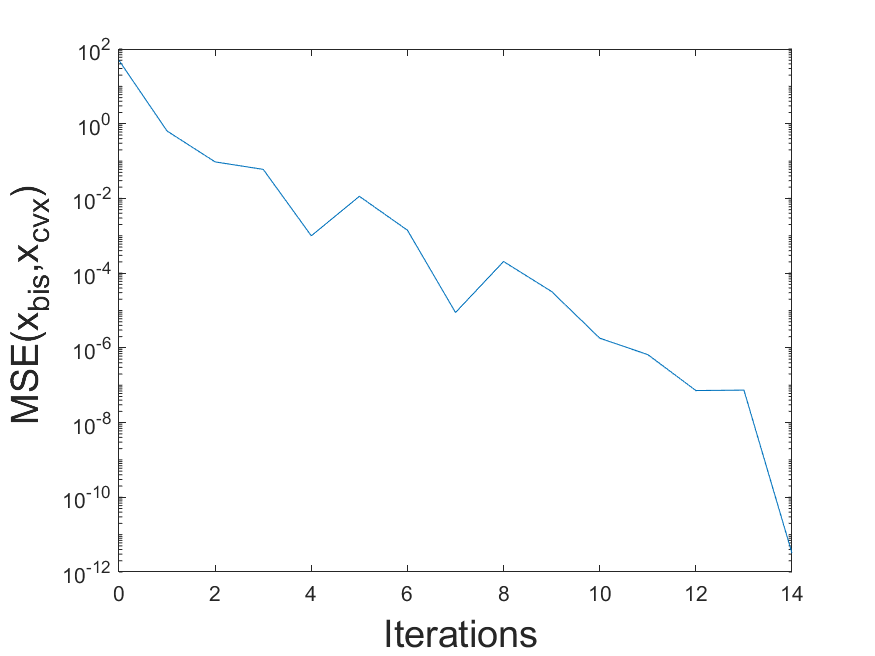
\includegraphics[width=0.7\textwidth]{P1-fig0.png}
				\caption{Mean Square Error Bisection Method-CVX, $err=10^{-4}$, $TOL=10^{-5}$}
			\end{figure}
			
			\newpage
		%%%%%%%%%%%%%%
		\item[\bf 2] Computation of a point in the set $S=S_1\cap S_2$ where,
		\begin{align*}
			S_1 = \{ {\bf x}\in\mathbb{R}^n | {\bf A}{\bf x}={\bf b} \}, \ S_2=\mathbb{R}^n_+
		\end{align*}
		
		Since the projection cant be easily calculated in closed form we will be using the alternating projection algorithm. 
		
		\begin{tcolorbox}
			{\bf Alternating Projection Algorithm}\\
			{\bf Initialization:} pick ${\bf x_0}\in\mathbb{R}^n$\\
			
			{\bf General Step:} for any $k=0,1,2,...$ execute: ${\bf x}_{k+1}=P_{S_2}(P_{S_1({\bf x}_k)})$
		\end{tcolorbox}
		The projections onto $S_1$ and $S_2$ respectively
		\begin{align*}
			&P_{S_1} = {\bf x}-{\bf A}^T({\bf A}{\bf A}^T)^{-1}({\bf A}{\bf x}-{\bf b})\\
			&P_{S_2} = [{\bf x}]_+	
		\end{align*}
		\begin{figure}[h]
			\centering
			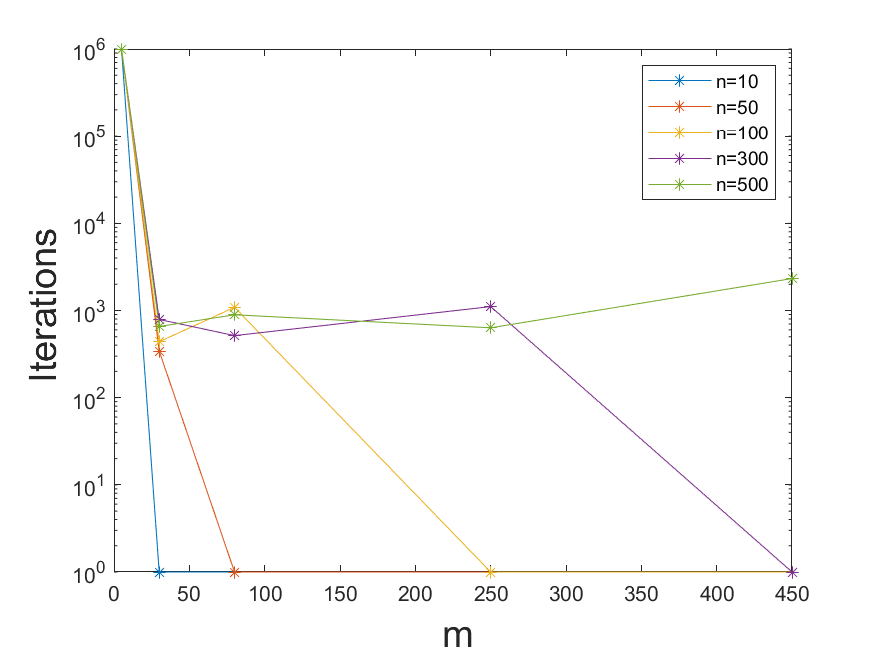
\includegraphics[width=\textwidth]{P2-fig2.png}
			\caption{Alternating Projection Algorithm m-Iterations for different n}
		\end{figure}
		
		We observe that for for small problem size the algorithm solves the problem in little iterations irrelevant to the $n-m$.\\
		As the problem size gets bigger the iterations increase. In this case we see that the algorithm runs faster when $n<<m$
		
		%%%%%%%%%%%%%%%
		\newpage
		\item[\bf 3] Let ${\bf c\in \mathbb{R}^n}$ and $\Delta_n=\{{\bf x}\in\mathbb{R}^n : {\bf x} \geq {\bf 0},{\bf e}^T{\bf x}=1\}$.\\
			The problem:
			\begin{align*}
				\begin{array}{c}
					\text{min }_{{\bf x\in \Delta_n}} f({\bf x})={\bf c}^T{\bf x}
				\end{array}
			\end{align*}
			Which can be written as:
			\begin{align*}
				&\text{min }_{{\bf x}\in \mathbb{R}^n} f({\bf x})={\bf c}^T{\bf x}\\
				&\begin{array}{cc}
					\text {s.t.}&h({\bf x})={\bf e}^T{\bf x} -1 = 0\\
					& f_i({\bf x})=-x_i\leq {\bf 0},\ i=1,...n
				\end{array}
			\end{align*}
		
			The KKT for this problem are:
			\begin{align*}
				&\nabla f({\bf x}) + \sum_i^n u_i\nabla f_i({\bf x}) + {\bf e}v = 0 \Rightarrow{\bf c} + {\bf u} + {\bf e}v = 0 \numberthis\\
				&u_i\geq0,\ i=1,...,n \numberthis\\
				&u_ix_i= 0,\ i=1,...n \numberthis\\
				&v\in\mathbb{R}
			\end{align*}
		
			\begin{figure}[h]
				\caption{Examples ${\bf c}^T{\bf x}$ Level Sets and the minimum on $\Delta_2$}
				\centering
				\begin{subfigure}[b]{0.4\textwidth}
					\centering
					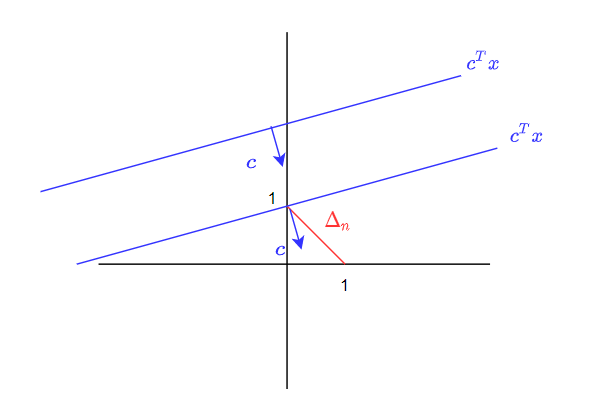
\includegraphics[width=\textwidth]{P3-fig0.png}
				\end{subfigure}
				\begin{subfigure}[b]{0.4\textwidth}
					\centering
					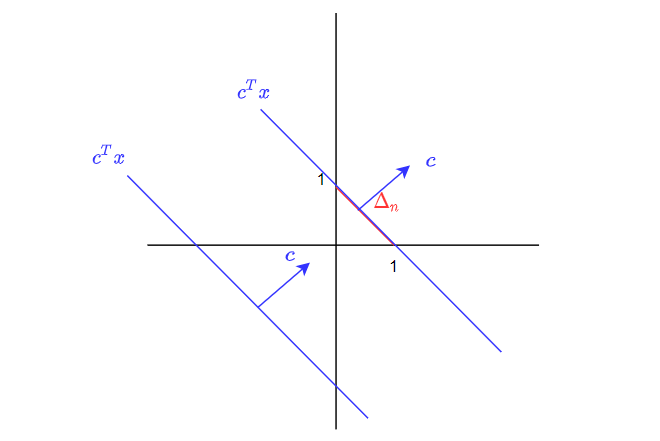
\includegraphics[width=\textwidth]{P3-fig1.png}
				\end{subfigure}
			\end{figure}
			
			As observed on the above examples we claim that a minimum ${\bf x^*}$ always has an element $x^*_k = 1,\ k=1,...,n$\\
			
			Therefore $x^*_k=1$, using (3): \\
			\begin{align*}
				&u_kx^*_k=0 \overset{x^*_k=1}{\Rightarrow}u_k=0\\
				&(1)\Rightarrow c_k + v=0 \iff v=-c_k\numberthis
			\end{align*}
			
			Replacing (4) in (1) an solving for ${\bf u}$ we get:
			\begin{align*}
				{\bf u} = {\bf e}c_k-{\bf c} \Rightarrow u_i = c_k-c_i,\ i=1,...,n\numberthis
			\end{align*}
		
			From (2) and (5) we get that: $\displaystyle c_i\geq c_k$.
			
			Therefore we can say that the solution ${\bf x^*}$ is 1 at $k = min_i{\{\bf c\}}$ and 0 at the other indices
			
			%%%%%%%%%%%%%%%%%%%%%%%
			\newpage
			\item[\bf 4]
		\end{enumerate}
\end{document}
